\documentclass[12pt,a4paper,oneside]{book}

\usepackage[utf8]{inputenc}
\usepackage[T1]{fontenc}
\usepackage{lmodern}
\usepackage{graphicx}
\usepackage{amsmath,amssymb}
\usepackage{geometry}
\usepackage{hyperref}
\usepackage{xcolor}
\usepackage{listings}
\usepackage{microtype}

% ---- Additional packages required for this report (diagrams, tables, figures) ----
\usepackage{tikz}
\usetikzlibrary{arrows.meta,positioning,shapes.geometric,shapes.multipart,calc,fit,backgrounds}
\usepackage{float}
\usepackage{booktabs}
\usepackage{array}
\usepackage{caption}
\usepackage{subcaption}
\usepackage{adjustbox}
\usepackage{titlesec}
\titleformat{\chapter}[display]{\normalfont\huge\bfseries}{}{0pt}{\Huge}% no ``Chapter 1'' label
\titlespacing*{\chapter}{0pt}{0pt}{20pt}

\geometry{margin=1in}
\emergencystretch=3em
\hypersetup{colorlinks=true,linkcolor=blue!50!black,urlcolor=blue!50!black,citecolor=blue!50!black}

% ---- C++ listing style ----
\lstdefinestyle{cpp}{
  language=C++,
  basicstyle=\ttfamily\footnotesize,
  keywordstyle=\color{blue!70!black}\bfseries,
  commentstyle=\color{green!45!black}\itshape,
  stringstyle=\color{red!60!black},
  numbers=left,
  numberstyle=\tiny\color{gray},
  numbersep=6pt,
  frame=single,
  rulecolor=\color{gray!60},
  backgroundcolor=\color{gray!5},
  breaklines=true,
  tabsize=4,
  showstringspaces=false,
  captionpos=b,
  xleftmargin=1.6em,
  framexleftmargin=1.3em,
  aboveskip=10pt,
  belowskip=6pt
}
\lstset{style=cpp}

% ---- Shared TikZ styles ----
\tikzset{
  stage/.style={draw, rounded corners=3pt, fill=blue!7, minimum width=8cm, minimum height=1.05cm, align=center, font=\small},
  io/.style={stage, fill=gray!15},
  flow/.style={-{Stealth[length=6pt]}, thick},
  % class diagram
  class/.style={rectangle split, rectangle split parts=3, draw, fill=white, font=\scriptsize\ttfamily,
                text width=5.2cm, align=left, inner xsep=3pt, inner ysep=2pt,
                rectangle split part fill={blue!12,white,white}},
  comp/.style={{Diamond[fill=black,length=10pt,width=6pt]}-, thick},
  aggr/.style={{Diamond[open,length=10pt,width=6pt]}-, thick},
  dep/.style={dashed, -{Stealth[open,length=7pt]}, thick},
  assoc/.style={-{Stealth[length=7pt]}, thick},
  gen/.style={-{Triangle[open,length=9pt,width=8pt]}, thick},
  rl/.style={font=\tiny, fill=white, inner sep=1pt},
  % activity diagrams
  act/.style={draw, rounded corners=7pt, fill=blue!6, text width=5.6cm, align=center, font=\small, minimum height=0.85cm},
  dec/.style={diamond, aspect=2.6, draw, fill=yellow!18, font=\footnotesize, inner sep=1pt, align=center},
  startn/.style={circle, fill=black, minimum size=0.4cm, inner sep=0pt},
  endn/.style={circle, draw, minimum size=0.55cm, inner sep=0pt,
               path picture={\fill (path picture bounding box.center) circle (0.17cm);}},
  aflow/.style={-{Stealth[length=6pt]}, thick},
  gl/.style={font=\scriptsize, fill=white, inner sep=1pt}
}

\makeatletter
\newcommand{\chapterauthor}[1]{%
  {\parindent0pt\vspace*{-15pt}%
  \linespread{1.1}\large\itshape\begin{flushright}#1\end{flushright}%
  \par\nobreak\vspace*{25pt}}
  \@afterheading%
}
\makeatother

% stick figure for the use case diagram
\newcommand{\stickman}[3]{%
  \draw[thick] (#1,#2) circle (0.22);
  \draw[thick] (#1,#2-0.22) -- (#1,#2-1.0);
  \draw[thick] (#1-0.4,#2-0.55) -- (#1+0.4,#2-0.55);
  \draw[thick] (#1,#2-1.0) -- (#1-0.3,#2-1.5);
  \draw[thick] (#1,#2-1.0) -- (#1+0.3,#2-1.5);
  \node[font=\small\bfseries, below, align=center] at (#1,#2-1.5) {#3};
}

% sequence diagram helpers
\newcommand{\smsg}[4]{\draw[-{Stealth[length=5pt]}] (#1,#3) -- node[above, font=\scriptsize, fill=white, inner sep=1pt, align=center] {#4} (#2,#3);}
\newcommand{\sret}[4]{\draw[dashed,-{Stealth[length=5pt,open]}] (#1,#3) -- node[above, font=\scriptsize, fill=white, inner sep=1pt, align=center] {#4} (#2,#3);}
\newcommand{\sself}[3]{\draw[-{Stealth[length=5pt]}] (#1,#2) -- ++(0.6,0) -- ++(0,-0.55) -- ++(-0.6,0);
  \node[anchor=west, font=\scriptsize, fill=white, inner sep=1pt, align=left] at (#1+0.65,#2-0.27) {#3};}

\begin{document}

\pagestyle{plain}% no running header; page number only
\mainmatter

% =====================================================================
% C++ OOP Mini-Project Chapter
% =====================================================================

\setcounter{chapter}{2}% next \chapter will be Chapter 3
\chapter{Object Tracking Engine}
\chapterauthor{Gautami Yeshwant Deshpande (251123)\\Abhipsa Mishra (251101)}

\begin{center}
\small
\begin{tabular}{@{}rl@{}}
\textbf{Guide:} & Dr.\ Anoop Jacob Thomas\\
\textbf{Department:} & Computer Science and Engineering\\
\textbf{Institute:} & Indian Institute of Information Technology, Tiruchirappalli\\
\textbf{Course stage:} & Second Year, Semester III (C++ OOP Mini-Project)
\end{tabular}
\end{center}
\vspace{4pt}

% =====================================================================
\section{Introduction and Problem Statement}
% =====================================================================
Detecting and following moving objects in video is a basic building block of video surveillance, traffic monitoring, sports analytics and robotics. A person watching a road camera can easily tell that ``the white car in the middle lane is moving forward quickly''; a program must reproduce that judgement from a grid of pixels, frame after frame.

The \textbf{Object Tracking Engine} is a C++17 desktop application that reads a video file, finds the moving objects in every frame, assigns each of them a persistent identity number, and reports how each one is moving: its speed, its direction of travel and whether it is moving or stationary. The results are shown on a live, annotated video window and also written to the console as a text log.

\subsection{Problem Statement}
Given a video stream, the system must:
\begin{enumerate}
    \item \textbf{detect} the regions of every frame that contain motion;
    \item \textbf{associate} detections in consecutive frames so that the same physical object keeps the same ID while it stays in view;
    \item \textbf{analyse} the motion of each tracked object (speed, direction, status); and
    \item \textbf{present} the result to the user visually and as text.
\end{enumerate}
The difficulty lies in the imperfect nature of real video: compression noise creates false detections, objects enter and leave the scene, and an object may be missed for a few frames. Besides a working result, the project aims at a clean object-oriented design in which every responsibility (reading frames, detecting, tracking, analysing, drawing) lives in its own class with a small, well-defined interface.

\subsection{What the System Does (End-User View)}
The user starts the program, optionally passing the path of a video file; if no path is given, \texttt{Video.mp4} in the working directory is used. A window titled ``Object Tracking Engine'' opens and plays the video. For every moving object the user sees:
\begin{itemize}
    \item a green rectangle around the object and a red dot at its centroid;
    \item a text label of the form \texttt{ID: <n> <STATUS> <DIRECTION> <speed> px/s}; and
    \item a blue line showing the path the object has followed so far.
\end{itemize}
At the same time, one log line per object per frame is printed to the console. Pressing \texttt{q} stops the program.

\subsection{Software Requirements}
\begin{table}[H]
\centering
\caption{Development and runtime environment}
\label{tab:env}
\small
\begin{tabular}{@{}p{3.6cm}p{11cm}@{}}
\toprule
\textbf{Item} & \textbf{Details}\\
\midrule
Language & C++17 (\texttt{CMAKE\_CXX\_STANDARD 17}, extensions off)\\
Library & OpenCV 5 (components: \texttt{core}, \texttt{geometry}, \texttt{imgproc}, \texttt{video}, \texttt{videoio}, \texttt{highgui})\\
Build system & CMake 3.16 or newer, with a \texttt{CMakePresets.json} preset for Visual Studio\\
Compiler & MSVC (enforced in \texttt{CMakeLists.txt} so that it matches the installed OpenCV binaries)\\
Platform & Windows, x64\\
Input & Any video format readable by OpenCV \texttt{videoio}; the demonstration uses a traffic-camera clip, \texttt{Video.mp4}\\
\bottomrule
\end{tabular}
\end{table}

% =====================================================================
\section{Scope and Feature Set}
% =====================================================================
\begin{itemize}
    \item \textbf{Moving-object detection:} Each frame is passed through an adaptive Gaussian-mixture background subtractor (MOG2). The foreground mask is cleaned with morphological opening and closing, and every sufficiently large connected region is reported as a \texttt{BoundingBox}.
    \item \textbf{Noise and size filtering:} Shadow pixels and weak foreground responses are removed by thresholding, small speckles by morphology, and regions smaller than a configurable minimum area (500 pixels by default) are discarded.
    \item \textbf{Persistent ID tracking:} Detections are matched to existing tracked objects by the distance between centroids (at most 80 pixels by default). Unmatched detections create new objects with fresh, increasing IDs.
    \item \textbf{Tolerance to missed detections:} An object that is not matched keeps its identity for up to five consecutive frames before it is deleted.
    \item \textbf{Motion analysis:} Speed (pixels per second, computed from real video timestamps), direction (\texttt{LEFT}, \texttt{RIGHT}, \texttt{UP}, \texttt{DOWN}, \texttt{STATIONARY}) and status (\texttt{MOVING} or \texttt{STATIONARY}) are computed for each object in every frame.
    \item \textbf{Visualisation:} Bounding box, centroid, text label and full trajectory are drawn on the frame. The display is scaled down automatically to fit within $1280\times720$ pixels.
    \item \textbf{Console logging:} The frame number, ID, position, speed, direction, status and missed-frame count of every object are printed for later inspection.
    \item \textbf{Configurable components:} The minimum area, matching distance, missed-frame limit and movement threshold are constructor parameters with sensible defaults.
    \item \textbf{Modular object-oriented design:} Seven cohesive classes with clear responsibilities, communicating through small, \texttt{const}-correct interfaces.
\end{itemize}

\paragraph{Out of scope.} The system does not convert pixel speeds to real-world units (no camera calibration), does not classify objects (car, bus, person), does not re-identify an object after a long disappearance, and does not save the annotated video to disk.

% =====================================================================
\section{Object-Oriented Architecture}
% =====================================================================
The design follows a few principles that recur throughout the code: \emph{encapsulation} (data members are private and exposed through \texttt{const} accessors), \emph{single responsibility} (each class does one job), \emph{composition} (larger objects own the smaller ones they are built from) and \emph{loose coupling} (classes exchange small value objects such as \texttt{Frame} and \texttt{BoundingBox} instead of sharing internal state).

\subsection{Overall Pipeline}
Figure~\ref{fig:pipeline} shows how data flows through the system for every frame. The \texttt{main()} function acts only as the coordinator: it owns one instance of each processing class and passes the output of one stage to the next.

\begin{figure}[H]
\centering
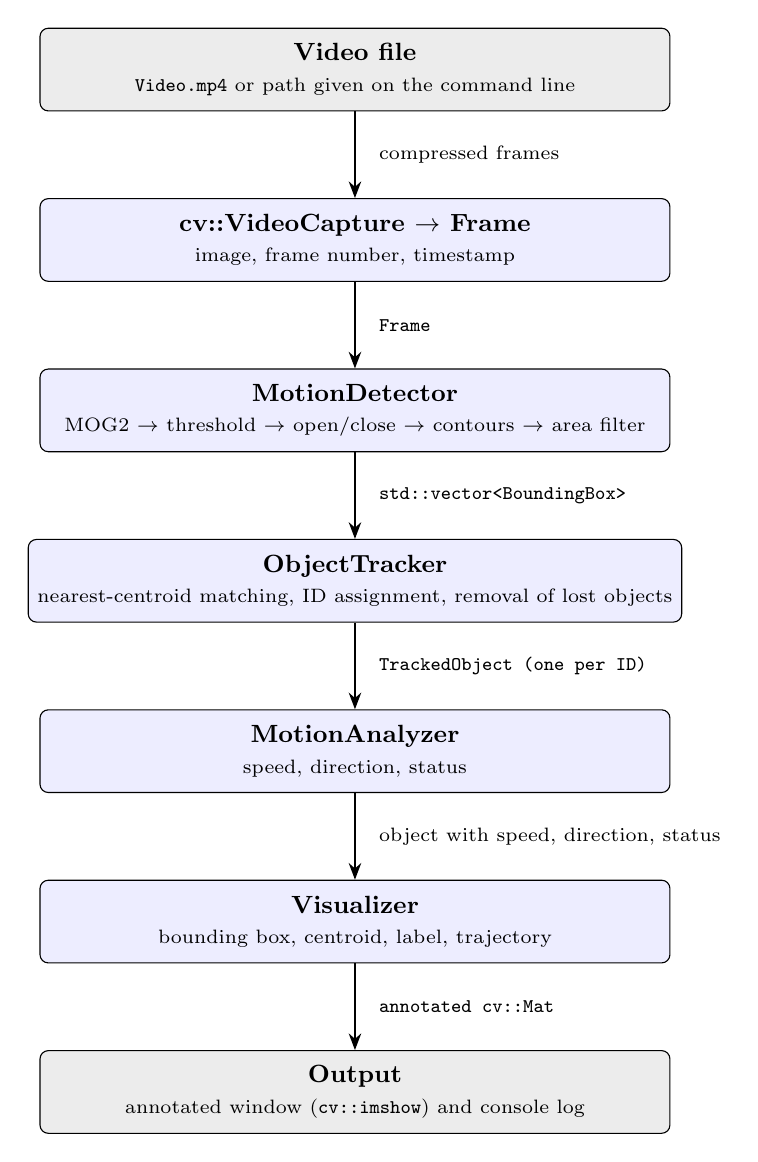
\begin{tikzpicture}
\node[io] (video) {\textbf{Video file}\\{\scriptsize \texttt{Video.mp4} or path given on the command line}};
\node[stage, below=1.1cm of video] (cap) {\textbf{cv::VideoCapture $\rightarrow$ Frame}\\{\scriptsize image, frame number, timestamp}};
\node[stage, below=1.1cm of cap] (det) {\textbf{MotionDetector}\\{\scriptsize MOG2 $\rightarrow$ threshold $\rightarrow$ open/close $\rightarrow$ contours $\rightarrow$ area filter}};
\node[stage, below=1.1cm of det] (trk) {\textbf{ObjectTracker}\\{\scriptsize nearest-centroid matching, ID assignment, removal of lost objects}};
\node[stage, below=1.1cm of trk] (ana) {\textbf{MotionAnalyzer}\\{\scriptsize speed, direction, status}};
\node[stage, below=1.1cm of ana] (vis) {\textbf{Visualizer}\\{\scriptsize bounding box, centroid, label, trajectory}};
\node[io, below=1.1cm of vis] (out) {\textbf{Output}\\{\scriptsize annotated window (\texttt{cv::imshow}) and console log}};
\draw[flow] (video) -- (cap) node[midway, right=5pt, font=\scriptsize] {compressed frames};
\draw[flow] (cap) -- (det) node[midway, right=5pt, font=\scriptsize\ttfamily] {Frame};
\draw[flow] (det) -- (trk) node[midway, right=5pt, font=\scriptsize\ttfamily] {std::vector<BoundingBox>};
\draw[flow] (trk) -- (ana) node[midway, right=5pt, font=\scriptsize\ttfamily] {TrackedObject (one per ID)};
\draw[flow] (ana) -- (vis) node[midway, right=5pt, font=\scriptsize] {object with speed, direction, status};
\draw[flow] (vis) -- (out) node[midway, right=5pt, font=\scriptsize\ttfamily] {annotated cv::Mat};
\end{tikzpicture}
\caption{Processing pipeline of the Object Tracking Engine (one iteration per video frame).}
\label{fig:pipeline}
\end{figure}

\subsection{Class Design and Associations}
The program consists of seven classes. Table~\ref{tab:classes} summarises their responsibilities and Figure~\ref{fig:class} shows the relations between them.

\begin{table}[H]
\centering
\caption{Classes and their responsibilities}
\label{tab:classes}
\small
\begin{tabular}{@{}p{3.1cm}p{7.2cm}p{4.7cm}@{}}
\toprule
\textbf{Class} & \textbf{Responsibility} & \textbf{Main collaborators}\\
\midrule
\texttt{Frame} & Immutable value object holding one video frame: a private copy of the image, its frame number and its timestamp in seconds. & \texttt{MotionDetector}, \texttt{main()}\\
\texttt{BoundingBox} & Axis-aligned rectangle ($x$, $y$, width, height) with centroid and area queries; supports \texttt{+} and \texttt{-} with a \texttt{cv::Point2f} offset. & \texttt{MotionDetector}, \texttt{TrackedObject}, \texttt{ObjectTracker}\\
\texttt{MotionDetector} & Finds moving regions in a frame using MOG2 background subtraction and contour analysis. & \texttt{Frame}, \texttt{BoundingBox}\\
\texttt{TrackedObject} & State of one tracked object: ID, current box, previous and current centroid, trajectory, timestamps, speed, direction, status and missed-frame counter. & \texttt{BoundingBox}\\
\texttt{ObjectTracker} & Maintains the collection of tracked objects; matches detections to objects, creates new objects and removes lost ones. & \texttt{TrackedObject}, \texttt{BoundingBox}\\
\texttt{MotionAnalyzer} & Computes speed, direction and status of a tracked object from its last two positions and timestamps. & \texttt{TrackedObject}\\
\texttt{Visualizer} & Draws the box, centroid, label and trajectory of an object onto a frame. & \texttt{TrackedObject}\\
\bottomrule
\end{tabular}
\end{table}

\begin{figure}[p]
\centering
\adjustbox{max width=\textwidth, max height=0.86\textheight}{%
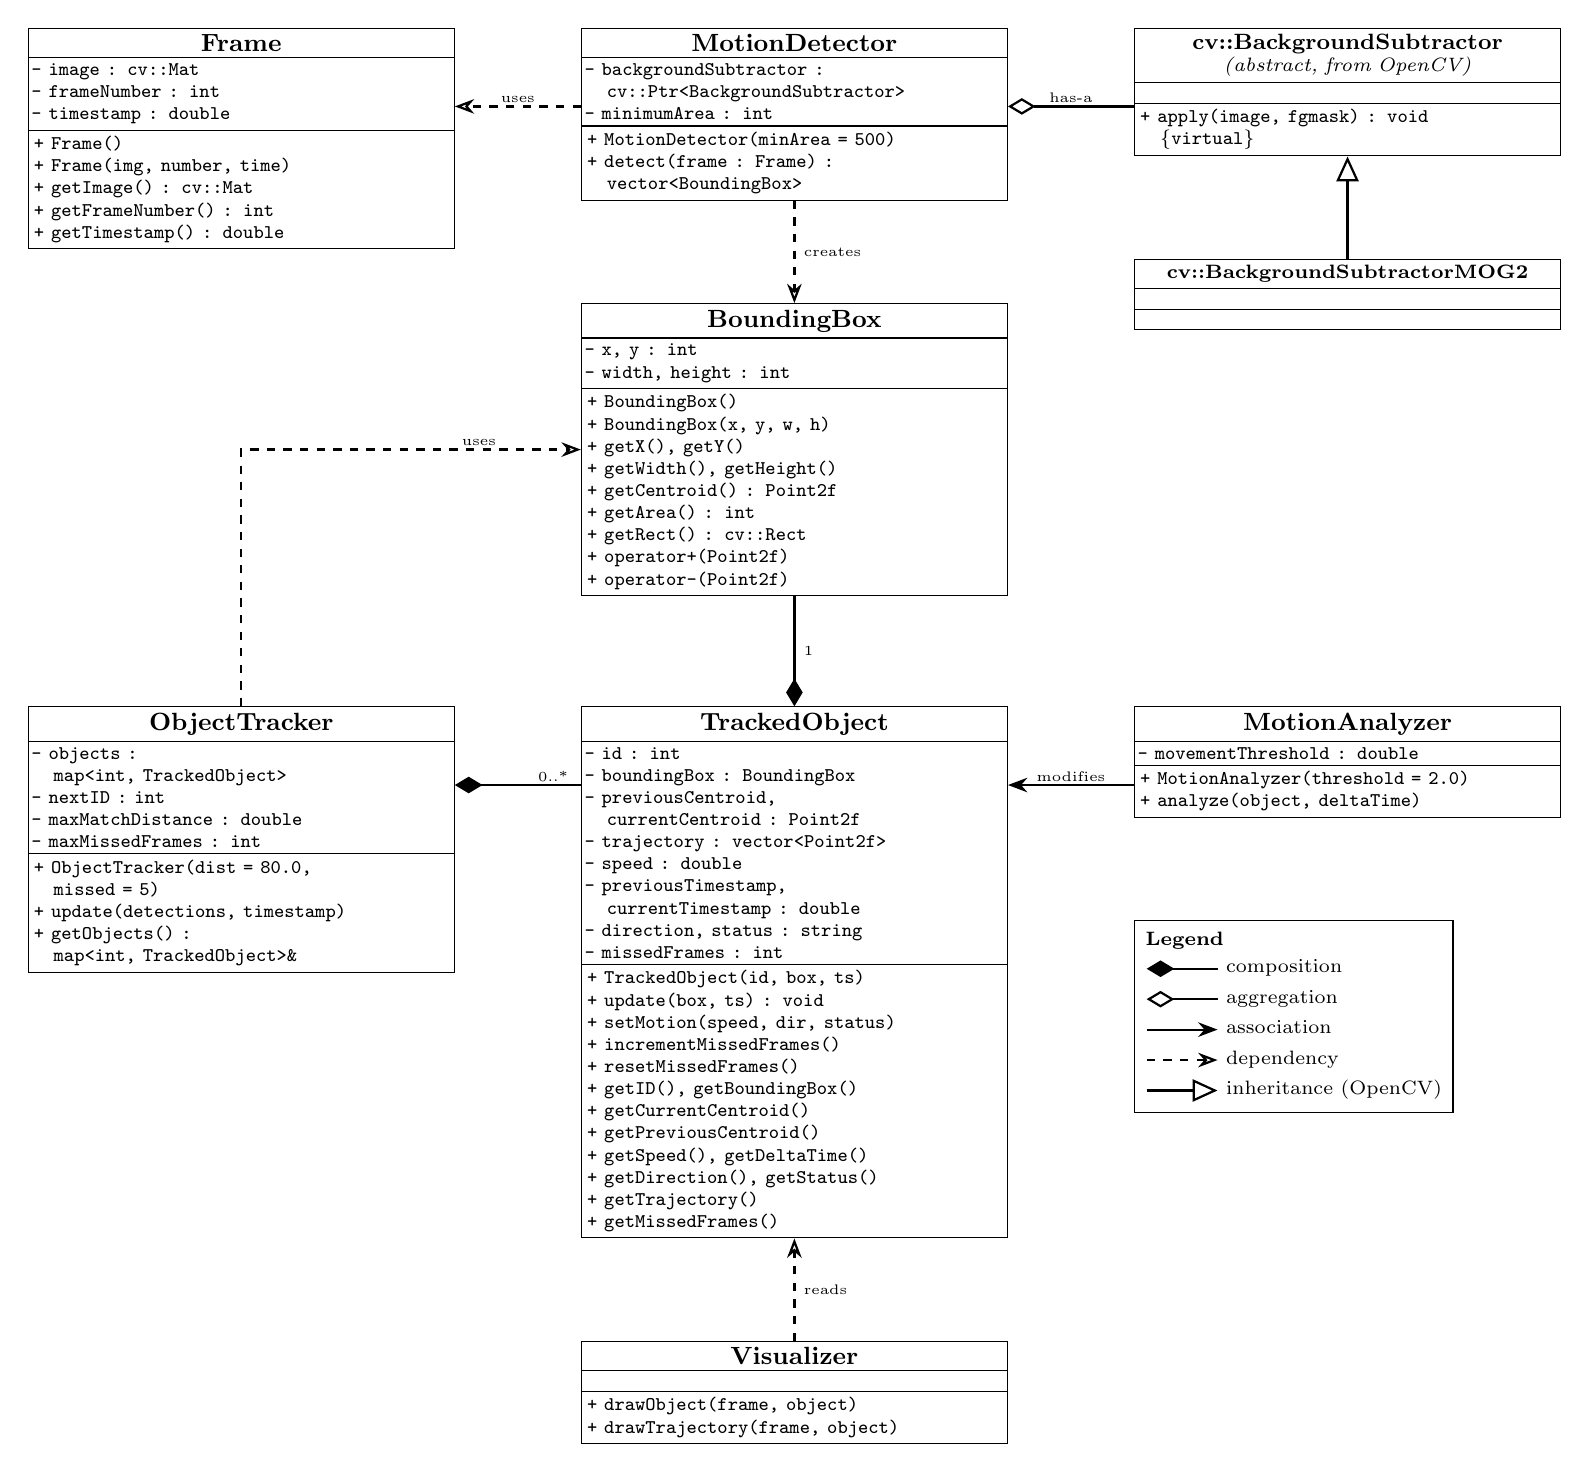
\begin{tikzpicture}
% ---------------- Row 1 ----------------
\node[class, anchor=north] (MD) at (0,0) {%
 \centerline{\rmfamily\bfseries\small MotionDetector}
 \nodepart{second}
 - backgroundSubtractor :\\
 \phantom{- }cv::Ptr<BackgroundSubtractor>\\
 - minimumArea : int
 \nodepart{third}
 + MotionDetector(minArea = 500)\\
 + detect(frame : Frame) :\\
 \phantom{+ }vector<BoundingBox>};
\node[class, anchor=north east] (FR) at ($(MD.north west)+(-1.6,0)$) {%
 \centerline{\rmfamily\bfseries\small Frame}
 \nodepart{second}
 - image : cv::Mat\\
 - frameNumber : int\\
 - timestamp : double
 \nodepart{third}
 + Frame()\\
 + Frame(img, number, time)\\
 + getImage() : cv::Mat\\
 + getFrameNumber() : int\\
 + getTimestamp() : double};
\node[class, anchor=north west] (BS) at ($(MD.north east)+(1.6,0)$) {%
 \centerline{\rmfamily\bfseries\footnotesize cv::BackgroundSubtractor}
 \centerline{\rmfamily\scriptsize\itshape (abstract, from OpenCV)}
 \nodepart{second}
 \phantom{x}
 \nodepart{third}
 + apply(image, fgmask) : void\\
 \phantom{+ }\{virtual\}};
% ---------------- Row 2 ----------------
\node[class, below=1.3cm of MD] (BB) {%
 \centerline{\rmfamily\bfseries\small BoundingBox}
 \nodepart{second}
 - x, y : int\\
 - width, height : int
 \nodepart{third}
 + BoundingBox()\\
 + BoundingBox(x, y, w, h)\\
 + getX(), getY()\\
 + getWidth(), getHeight()\\
 + getCentroid() : Point2f\\
 + getArea() : int\\
 + getRect() : cv::Rect\\
 + operator+(Point2f)\\
 + operator-(Point2f)};
\node[class, below=1.3cm of BS] (MOG) {%
 \centerline{\rmfamily\bfseries\scriptsize cv::BackgroundSubtractorMOG2}
 \nodepart{second}
 \phantom{x}
 \nodepart{third}
 \phantom{x}};
% ---------------- Row 3 ----------------
\node[class, below=1.4cm of BB] (TO) {%
 \centerline{\rmfamily\bfseries\small TrackedObject}
 \nodepart{second}
 - id : int\\
 - boundingBox : BoundingBox\\
 - previousCentroid,\\
 \phantom{- }currentCentroid : Point2f\\
 - trajectory : vector<Point2f>\\
 - speed : double\\
 - previousTimestamp,\\
 \phantom{- }currentTimestamp : double\\
 - direction, status : string\\
 - missedFrames : int
 \nodepart{third}
 + TrackedObject(id, box, ts)\\
 + update(box, ts) : void\\
 + setMotion(speed, dir, status)\\
 + incrementMissedFrames()\\
 + resetMissedFrames()\\
 + getID(), getBoundingBox()\\
 + getCurrentCentroid()\\
 + getPreviousCentroid()\\
 + getSpeed(), getDeltaTime()\\
 + getDirection(), getStatus()\\
 + getTrajectory()\\
 + getMissedFrames()};
\node[class, anchor=north east] (OT) at ($(TO.north west)+(-1.6,0)$) {%
 \centerline{\rmfamily\bfseries\small ObjectTracker}
 \nodepart{second}
 - objects :\\
 \phantom{- }map<int, TrackedObject>\\
 - nextID : int\\
 - maxMatchDistance : double\\
 - maxMissedFrames : int
 \nodepart{third}
 + ObjectTracker(dist = 80.0,\\
 \phantom{+ }missed = 5)\\
 + update(detections, timestamp)\\
 + getObjects() :\\
 \phantom{+ }map<int, TrackedObject>\&};
\node[class, anchor=north west] (MA) at ($(TO.north east)+(1.6,0)$) {%
 \centerline{\rmfamily\bfseries\small MotionAnalyzer}
 \nodepart{second}
 - movementThreshold : double
 \nodepart{third}
 + MotionAnalyzer(threshold = 2.0)\\
 + analyze(object, deltaTime)};
% ---------------- Row 4 ----------------
\node[class, below=1.3cm of TO] (VI) {%
 \centerline{\rmfamily\bfseries\small Visualizer}
 \nodepart{second}
 \phantom{x}
 \nodepart{third}
 + drawObject(frame, object)\\
 + drawTrajectory(frame, object)};
% ---------------- Relationships ----------------
% MotionDetector uses Frame
\draw[dep] ($(MD.north west)+(0,-1.0)$) -- node[rl, above] {uses} ($(FR.north east)+(0,-1.0)$);
% MotionDetector aggregates BackgroundSubtractor (shared ownership via cv::Ptr)
\draw[aggr] ($(MD.north east)+(0,-1.0)$) -- node[rl, above] {has-a} ($(BS.north west)+(0,-1.0)$);
% MOG2 inherits BackgroundSubtractor
\draw[gen] (MOG.north) -- (BS.south);
% MotionDetector creates BoundingBox
\draw[dep] (MD.south) -- node[rl, right=2pt] {creates} (BB.north);
% TrackedObject composes BoundingBox
\draw[comp] (TO.north) -- node[rl, right=2pt, pos=0.5] {1} (BB.south);
% ObjectTracker composes TrackedObject
\draw[comp] ($(OT.north east)+(0,-1.0)$) -- node[rl, above, pos=0.78] {0..*} ($(TO.north west)+(0,-1.0)$);
% ObjectTracker uses BoundingBox
\draw[dep] (OT.north) |- node[rl, above, pos=0.85] {uses} (BB.west);
% MotionAnalyzer modifies TrackedObject
\draw[assoc] ($(MA.north west)+(0,-1.0)$) -- node[rl, above] {modifies} ($(TO.north east)+(0,-1.0)$);
% Visualizer reads TrackedObject
\draw[dep] (VI.north) -- node[rl, right=2pt] {reads} (TO.south);
% ---------------- Legend ----------------
\node[draw, fill=white, font=\scriptsize, anchor=north west, align=left, inner sep=4pt] (LG) at ($(MA.south west)+(0,-1.3)$) {%
 \textbf{Legend}\\[2pt]
 \tikz[baseline=-0.5ex]{\draw[comp] (0,0) -- (0.9,0);} composition\\[3pt]
 \tikz[baseline=-0.5ex]{\draw[aggr] (0,0) -- (0.9,0);} aggregation\\[3pt]
 \tikz[baseline=-0.5ex]{\draw[assoc] (0,0) -- (0.9,0);} association\\[3pt]
 \tikz[baseline=-0.5ex]{\draw[dep] (0,0) -- (0.9,0);} dependency\\[3pt]
 \tikz[baseline=-0.5ex]{\draw[gen] (0,0) -- (0.9,0);} inheritance (OpenCV)};
\end{tikzpicture}}
\caption{UML class diagram. The seven project classes are linked by composition, association and dependency; the only inheritance involved belongs to OpenCV's background-subtractor interface.}
\label{fig:class}
\end{figure}

\paragraph{Composition.}
\texttt{TrackedObject} \emph{owns} its \texttt{BoundingBox} and its trajectory (a \texttt{std::\allowbreak vector<\allowbreak cv::\allowbreak Point2f>}) as ordinary data members; they cannot exist without the object. \texttt{ObjectTracker} owns every \texttt{TrackedObject} by value inside a \texttt{std::map<int, TrackedObject>}: when the tracker erases an entry, the object and everything it contains are destroyed with it. Likewise \texttt{Frame} owns a private deep copy of its image.

\paragraph{Aggregation.}
\texttt{MotionDetector} holds its background model through a \texttt{cv::\allowbreak Ptr<\allowbreak cv::\allowbreak BackgroundSubtractor>}, a reference-counted smart pointer. The detector uses the subtractor as a part of itself, but the part is managed by shared ownership rather than embedded by value, which is why it is drawn as aggregation.

\paragraph{Association and dependency.}
\texttt{MotionAnalyzer} receives a \texttt{TrackedObject} by non-\texttt{const} reference and updates it through \texttt{setMotion()}. \texttt{Visualizer} only reads a \texttt{TrackedObject}. \texttt{MotionDetector} depends on \texttt{Frame} (its input) and creates \texttt{BoundingBox} values (its output), and \texttt{ObjectTracker} depends on \texttt{BoundingBox} for the detections it receives. These are short-lived ``uses'' relations; none of the classes stores a long-term pointer to another.

\paragraph{Inheritance.}
The project does not define its own class hierarchy, because the problem is naturally a chain of independent processing steps rather than a family of related types. Inheritance and run-time polymorphism enter only through OpenCV: \texttt{MotionDetector} calls \texttt{apply()} through a pointer to the abstract base class \texttt{cv::BackgroundSubtractor}, while the object behind it is a \texttt{BackgroundSubtractorMOG2} (Section~\ref{sec:polymorphism}).

% =====================================================================
\section{OOP Concepts Demonstrated in the Code}
\label{sec:oop}
% =====================================================================
This section shows, using the actual source code, how the main object-oriented concepts are applied.

\subsection{Encapsulation and Data Hiding}
Every class keeps its data private and offers read access through \texttt{const} member functions. \texttt{BoundingBox} is a typical example: no outside code can put it in an inconsistent state, and the derived values (centroid, area, \texttt{cv::Rect}) are computed on demand rather than stored.

\begin{lstlisting}[caption={\texttt{BoundingBox.h}: private data, public \texttt{const} interface.}, label={lst:bbox-h}]
class BoundingBox
{
private:
    int x;
    int y;
    int width;
    int height;

public:
    BoundingBox();
    BoundingBox(int x, int y, int width, int height);

    int getX() const;
    int getY() const;
    int getWidth() const;
    int getHeight() const;

    cv::Point2f getCentroid() const;
    int getArea() const;
    cv::Rect getRect() const;

    // Operator overloading
    BoundingBox operator+(const cv::Point2f& offset) const;
    BoundingBox operator-(const cv::Point2f& offset) const;
};
\end{lstlisting}

\texttt{TrackedObject} goes one step further: its state can only change through the controlled operations \texttt{update()}, \texttt{setMotion()}, \texttt{incrementMissedFrames()} and \texttt{resetMissedFrames()}. In particular, \texttt{update()} guarantees that the previous and current centroids and timestamps always move forward together, which the analyser relies on.

\begin{lstlisting}[caption={\texttt{TrackedObject::update()} keeps position, time and history consistent.}, label={lst:update}]
void TrackedObject::update(const BoundingBox& newBox, double timestamp)
{
    previousCentroid = currentCentroid;
    previousTimestamp = currentTimestamp;
    currentTimestamp = timestamp;

    boundingBox = newBox;
    currentCentroid = newBox.getCentroid();
    trajectory.push_back(currentCentroid);

    missedFrames = 0;
}
\end{lstlisting}

\subsection{Constructors and Constructor Overloading}
\texttt{BoundingBox} provides a default constructor (an empty box at the origin) and a parameterised one. \texttt{Frame} does the same. In \texttt{Frame}, the parameterised constructor calls \texttt{clone()} on the image, so the \texttt{Frame} owns an independent copy: later drawing on the original image in \texttt{main()} cannot affect the data that the detector processes.

\begin{lstlisting}[caption={Overloaded constructors of \texttt{BoundingBox} and \texttt{Frame}.}, label={lst:ctor}]
BoundingBox::BoundingBox()
{
    x = 0;
    y = 0;
    width = 0;
    height = 0;
}

BoundingBox::BoundingBox(int x, int y, int width, int height)
{
    this->x = x;
    this->y = y;
    this->width = width;
    this->height = height;
}

Frame::Frame(const cv::Mat& img, int number, double time)
{
    image = img.clone();
    frameNumber = number;
    timestamp = time;
}
\end{lstlisting}

\subsection{Default Arguments}
The tunable classes take their parameters through constructors with default values, so a component can be created with a recommended configuration or customised at the call site. In \texttt{main()} the defaults are overridden explicitly: \texttt{MotionDetector detector(500);}, \texttt{ObjectTracker tracker(80.0, 5);} and \texttt{MotionAnalyzer analyzer(2.0);}.

\begin{lstlisting}[caption={Constructors with default arguments (declarations).}, label={lst:default}]
MotionDetector(int minArea = 500);                 // MotionDetector.h
MotionAnalyzer(double threshold = 2.0);            // MotionAnalyzer.h
ObjectTracker(double maxDistance = 80.0,           // Tracker.h
              int maxMissed = 5);
TrackedObject(int id, const BoundingBox& box,      // TrackedObject.h
              double timestamp = 0.0);
\end{lstlisting}

\subsection{Operator Overloading}
\texttt{BoundingBox} overloads \texttt{+} and \texttt{-} so that a box can be translated by a \texttt{cv::Point2f} offset with natural syntax: \texttt{BoundingBox moved = box + offset;}. Both operators are \texttt{const} and return a new box, leaving the original unchanged; the size is preserved. The floating-point offset is truncated to whole pixels because the box stores integer coordinates.

\begin{lstlisting}[caption={Overloaded \texttt{+} and \texttt{-} operators, and the centroid computation.}, label={lst:operators}]
cv::Point2f BoundingBox::getCentroid() const
{
    return cv::Point2f(
        x + width / 2.0f,
        y + height / 2.0f
    );
}

BoundingBox BoundingBox::operator+(const cv::Point2f& offset) const
{
    return BoundingBox(
        x + static_cast<int>(offset.x),
        y + static_cast<int>(offset.y),
        width,
        height
    );
}

BoundingBox BoundingBox::operator-(const cv::Point2f& offset) const
{
    return BoundingBox(
        x - static_cast<int>(offset.x),
        y - static_cast<int>(offset.y),
        width,
        height
    );
}
\end{lstlisting}

\subsection{Composition and Ownership of Objects}
The tracker is the clearest example of composition. It owns all tracked objects in a \texttt{std::map} keyed by ID; \texttt{nextID} guarantees that IDs are never reused during a run. Because the objects are stored by value, creation and destruction of a \texttt{TrackedObject} are tied to the tracker's own bookkeeping, with no manual \texttt{new} or \texttt{delete} anywhere in the project.

\begin{lstlisting}[caption={\texttt{Tracker.h}: \texttt{ObjectTracker} owns its \texttt{TrackedObject}s.}, label={lst:tracker-h}]
class ObjectTracker
{
private:
    std::map<int, TrackedObject> objects;

    int nextID;

    double maxMatchDistance;
    int maxMissedFrames;

public:
    ObjectTracker(double maxDistance = 80.0, int maxMissed = 5);

    void update(const std::vector<BoundingBox>& detections,
                double timestamp = 0.0);

    std::map<int, TrackedObject>& getObjects();
};
\end{lstlisting}

\subsection{Abstraction and Separation of Responsibilities}
Each stage of the pipeline is hidden behind a one- or two-function interface. The caller does not need to know that detection uses MOG2 or that matching is greedy; it only needs \texttt{detect()}, \texttt{update()}, \texttt{analyze()} and \texttt{draw*()}. This makes it possible to replace the internals of one class (for example, a better matching algorithm in \texttt{ObjectTracker}) without touching the others. The main loop below reads almost like the problem statement.

\begin{lstlisting}[caption={Core of the main loop: each stage is a single call on a dedicated object.}, label={lst:main}]
Frame frame(image, frameNumber, timestamp);
// 1. Detect moving objects
std::vector<BoundingBox> detections = detector.detect(frame);
// 2. Track objects
tracker.update(detections, timestamp);
// 3. Analyze and visualize
for (auto& pair : tracker.getObjects()) {
    TrackedObject& object = pair.second;
    analyzer.analyze(object, object.getDeltaTime());
    visualizer.drawObject(image, object);
    visualizer.drawTrajectory(image, object);
    // ... console log ...
}
\end{lstlisting}

\subsection{Const-Correctness}
Accessors are declared \texttt{const}, inputs are passed as \texttt{const} references (\texttt{const BoundingBox\&}, \texttt{const Frame\&}, \texttt{const TrackedObject\&}), and the trajectory is exposed as a \texttt{const std::vector<cv::Point2f>\&} to avoid copying a growing vector. For instance, \texttt{MotionDetector::detect(const Frame\&)} promises not to modify the frame, and \texttt{Visualizer::drawObject()} takes the object as \texttt{const}, documenting that drawing never changes tracking state. Only \texttt{MotionAnalyzer::analyze()} receives a modifiable \texttt{TrackedObject\&}, which makes it easy to see which class is allowed to change motion data.

\subsection{Polymorphism through an Abstract Interface and RAII}
\label{sec:polymorphism}
\texttt{MotionDetector} stores its background model as a \texttt{cv::\allowbreak Ptr<\allowbreak cv::\allowbreak BackgroundSubtractor>} (the abstract base class) and initialises it with the MOG2 implementation. The call to \texttt{apply()} is dispatched at run time to \texttt{BackgroundSubtractorMOG2}, so the detector would work unchanged with another subtractor such as KNN. The smart pointer also illustrates RAII: the model is released automatically when the detector is destroyed, just as \texttt{cv::Mat} images and the \texttt{cv::VideoCapture} release their resources without explicit clean-up code.

\begin{lstlisting}[caption={Programming to the abstract \texttt{cv::BackgroundSubtractor} interface.}, label={lst:poly}]
// MotionDetector.h
cv::Ptr<cv::BackgroundSubtractor> backgroundSubtractor;

// MotionDetector.cpp
MotionDetector::MotionDetector(int minArea)
{
    minimumArea = minArea;
    backgroundSubtractor = cv::createBackgroundSubtractorMOG2();
}
...
backgroundSubtractor->apply(image, foregroundMask);   // virtual call
\end{lstlisting}

\begin{table}[H]
\centering
\caption{Where each OOP concept appears in the project}
\label{tab:oop-map}
\small
\begin{tabular}{@{}p{4.2cm}p{10.8cm}@{}}
\toprule
\textbf{Concept} & \textbf{Location in the code}\\
\midrule
Encapsulation & Private members and \texttt{const} getters in \texttt{BoundingBox}, \texttt{Frame}, \texttt{TrackedObject}\\
Constructor overloading & \texttt{BoundingBox()} / \texttt{BoundingBox(x,y,w,h)}; \texttt{Frame()} / \texttt{Frame(img,n,t)}\\
Default arguments & \texttt{MotionDetector}, \texttt{MotionAnalyzer}, \texttt{ObjectTracker}, \texttt{TrackedObject} constructors\\
Operator overloading & \texttt{BoundingBox::operator+} and \texttt{operator-}\\
Composition & \texttt{ObjectTracker} $\rightarrow$ \texttt{TrackedObject} $\rightarrow$ \texttt{BoundingBox}; \texttt{Frame} $\rightarrow$ image copy\\
Aggregation (shared ownership) & \texttt{MotionDetector} $\rightarrow$ \texttt{cv::Ptr<BackgroundSubtractor>}\\
Abstraction / single responsibility & Seven classes with narrow public interfaces, coordinated by \texttt{main()}\\
Const-correctness & \texttt{const} member functions and \texttt{const} reference parameters throughout\\
Polymorphism (via OpenCV) & \texttt{BackgroundSubtractor::apply()} called through a base-class smart pointer\\
RAII / automatic resource management & \texttt{cv::Ptr}, \texttt{cv::Mat}, \texttt{std::map}, \texttt{std::vector}; no raw \texttt{new}/\texttt{delete}\\
\bottomrule
\end{tabular}
\end{table}

% =====================================================================
\section{UML Behavioural Models}
% =====================================================================

\subsection{Use Case Diagram}
Figure~\ref{fig:usecase} shows the interactions between the user, the video source and the system. The \emph{User} starts the tracker, views the annotated video, reads the console log and quits. The \emph{Video file} is a secondary actor that supplies frames. Internally, annotating the video requires motion analysis, which requires tracking, which requires detection, which requires reading frames; this chain is expressed with \emph{include} relations.

\begin{figure}[H]
\centering
\adjustbox{max width=\textwidth}{%
\begin{tikzpicture}[
  uc/.style={ellipse, draw, fill=blue!6, minimum height=1.1cm, text width=3.1cm, align=center, font=\scriptsize, inner sep=1pt},
  inc/.style={dashed, -{Stealth[length=5pt,open]}}
]
% system boundary
\draw[rounded corners=4pt, thick] (2.2,-5.2) rectangle (12.4,7.0);
\node[font=\small\bfseries, anchor=north] at (7.3,6.95) {Object Tracking Engine};
% actors
\stickman{0.3}{1.2}{User}
\stickman{14.3}{6.1}{Video file}
% middle column (user goals)
\node[uc] (U1) at (4.1,5.5) {Start tracking\\(optional video path)};
\node[uc] (U4) at (4.1,3.3) {Quit (press \texttt{q})};
\node[uc] (U3) at (4.1,-1.1) {Read console motion log};
\node[uc] (U2) at (4.1,-3.3) {View annotated video};
% right column (included behaviour)
\node[uc] (R1) at (10.0,5.5) {Read video frames};
\node[uc] (R2) at (10.0,3.3) {Detect moving objects};
\node[uc] (R3) at (10.0,1.1) {Track objects (persistent IDs)};
\node[uc] (R4) at (10.0,-1.1) {Analyze motion (speed, direction, status)};
\node[uc] (R5) at (10.0,-3.3) {Draw boxes, labels and trajectories};
% associations
\foreach \u in {U1,U4,U3,U2} \draw[thick] (0.75,0.65) -- (\u.west);
\draw[thick] (R1.east) -- (13.85,5.5);
% include relations
\draw[inc] (U1.east) -- node[above, font=\tiny] {\guillemotleft include\guillemotright} (R1.west);
\draw[inc] (U3.east) -- node[above, font=\tiny] {\guillemotleft include\guillemotright} (R4.west);
\draw[inc] (U2.east) -- node[above, font=\tiny] {\guillemotleft include\guillemotright} (R5.west);
\draw[inc] (R5.north) -- node[right, font=\tiny] {\guillemotleft include\guillemotright} (R4.south);
\draw[inc] (R4.north) -- node[right, font=\tiny] {\guillemotleft include\guillemotright} (R3.south);
\draw[inc] (R3.north) -- node[right, font=\tiny] {\guillemotleft include\guillemotright} (R2.south);
\draw[inc] (R2.north) -- node[right, font=\tiny] {\guillemotleft include\guillemotright} (R1.south);
\end{tikzpicture}}
\caption{Use case diagram of the Object Tracking Engine.}
\label{fig:usecase}
\end{figure}

\subsection{Sequence Diagram}
Figure~\ref{fig:sequence} shows the messages exchanged while one frame is processed. \texttt{main()} reads the frame and wraps it in a \texttt{Frame}, asks the detector for bounding boxes, hands them to the tracker (which updates, creates or ages \texttt{TrackedObject}s), and finally, for every tracked object, calls the analyser and the visualiser, both of which talk to the \texttt{TrackedObject}.

\begin{figure}[p]
\centering
\adjustbox{max width=\textwidth, max height=0.86\textheight}{%
\begin{tikzpicture}[
  life/.style={draw, fill=blue!8, minimum width=2.2cm, minimum height=0.7cm, font=\scriptsize\ttfamily, align=center},
  frag/.style={draw, thick, gray!70!black},
  ftab/.style={draw, fill=white, font=\tiny\bfseries, inner sep=2pt, anchor=north west}
]
% lifelines
\node[life] (main) at (0,0)    {main()};
\node[life] (md)   at (2.9,0)  {:MotionDetector};
\node[life] (ot)   at (5.8,0)  {:ObjectTracker};
\node[life] (to)   at (8.7,0)  {:TrackedObject};
\node[life] (ma)   at (11.6,0) {:MotionAnalyzer};
\node[life] (vi)   at (14.5,0) {:Visualizer};
\foreach \n in {main,md,ot,to,ma,vi} \draw[dashed, gray] (\n.south) -- ++(0,-22.6);
% 1. read frame and build Frame
\sself{0}{-1.0}{video.read(image);\\Frame frame(image, n, ts)}
% 2. detect
\smsg{0}{2.9}{-2.4}{detect(frame)}
\sself{2.9}{-2.9}{MOG2, threshold,\\morphology, contours}
\sret{2.9}{0}{-4.2}{detections}
% 3. tracker update
\smsg{0}{5.8}{-5.2}{update(detections, timestamp)}
\draw[frag] (5.0,-5.7) rectangle (9.5,-9.4);
\node[ftab] at (5.0,-5.7) {loop};
\node[font=\tiny, anchor=north west] at (5.55,-5.7) {[for each object / detection]};
\smsg{5.8}{8.7}{-6.9}{update(box, ts)\\{[matched]}}
\smsg{5.8}{8.7}{-7.9}{incrementMissedFrames()\\{[no match]}}
\smsg{5.8}{8.7}{-8.9}{\guillemotleft create\guillemotright (id, box, ts)\\{[unmatched detection]}}
\sself{5.8}{-9.8}{erase if missed\\$>$ maxMissedFrames}
% 4. get objects
\smsg{0}{5.8}{-11.2}{getObjects()}
\sret{5.8}{0}{-12.0}{map<int, TrackedObject>\&}
% 5. per-object processing
\draw[frag] (-0.8,-12.7) rectangle (15.4,-21.9);
\node[ftab] at (-0.8,-12.7) {loop};
\node[font=\tiny, anchor=north west] at (-0.25,-12.7) {[for each (id, object) in map]};
\smsg{0}{11.6}{-13.9}{analyze(object, deltaTime)}
\smsg{11.6}{8.7}{-14.8}{getPreviousCentroid()\\getCurrentCentroid()}
\smsg{11.6}{8.7}{-15.9}{setMotion(speed,\\direction, status)}
\smsg{0}{14.5}{-17.0}{drawObject(image, object)}
\smsg{14.5}{8.7}{-17.9}{getBoundingBox(), getCurrentCentroid(),\\getID(), getStatus(), getDirection(), getSpeed()}
\smsg{0}{14.5}{-19.0}{drawTrajectory(image, object)}
\smsg{14.5}{8.7}{-19.8}{getTrajectory()}
\smsg{0}{8.7}{-21.0}{console log: getID(), getCurrentCentroid(), getSpeed(),\\getDirection(), getStatus(), getMissedFrames()}
% 6. display
\sself{0}{-22.3}{cv::resize(); cv::imshow();\\cv::waitKey(1)}
\end{tikzpicture}}
\caption{Sequence diagram for processing one video frame (simplified: object creation and the missed-frame bookkeeping are shown for one object only).}
\label{fig:sequence}
\end{figure}

\subsection{Activity Diagrams}
Figure~\ref{fig:activity-main} describes the control flow of the application as a whole, and Figure~\ref{fig:activity-tracker} zooms into the matching logic inside \texttt{ObjectTracker::update()}.

\begin{figure}[p]
\centering
\adjustbox{max width=\textwidth, max height=0.86\textheight}{%
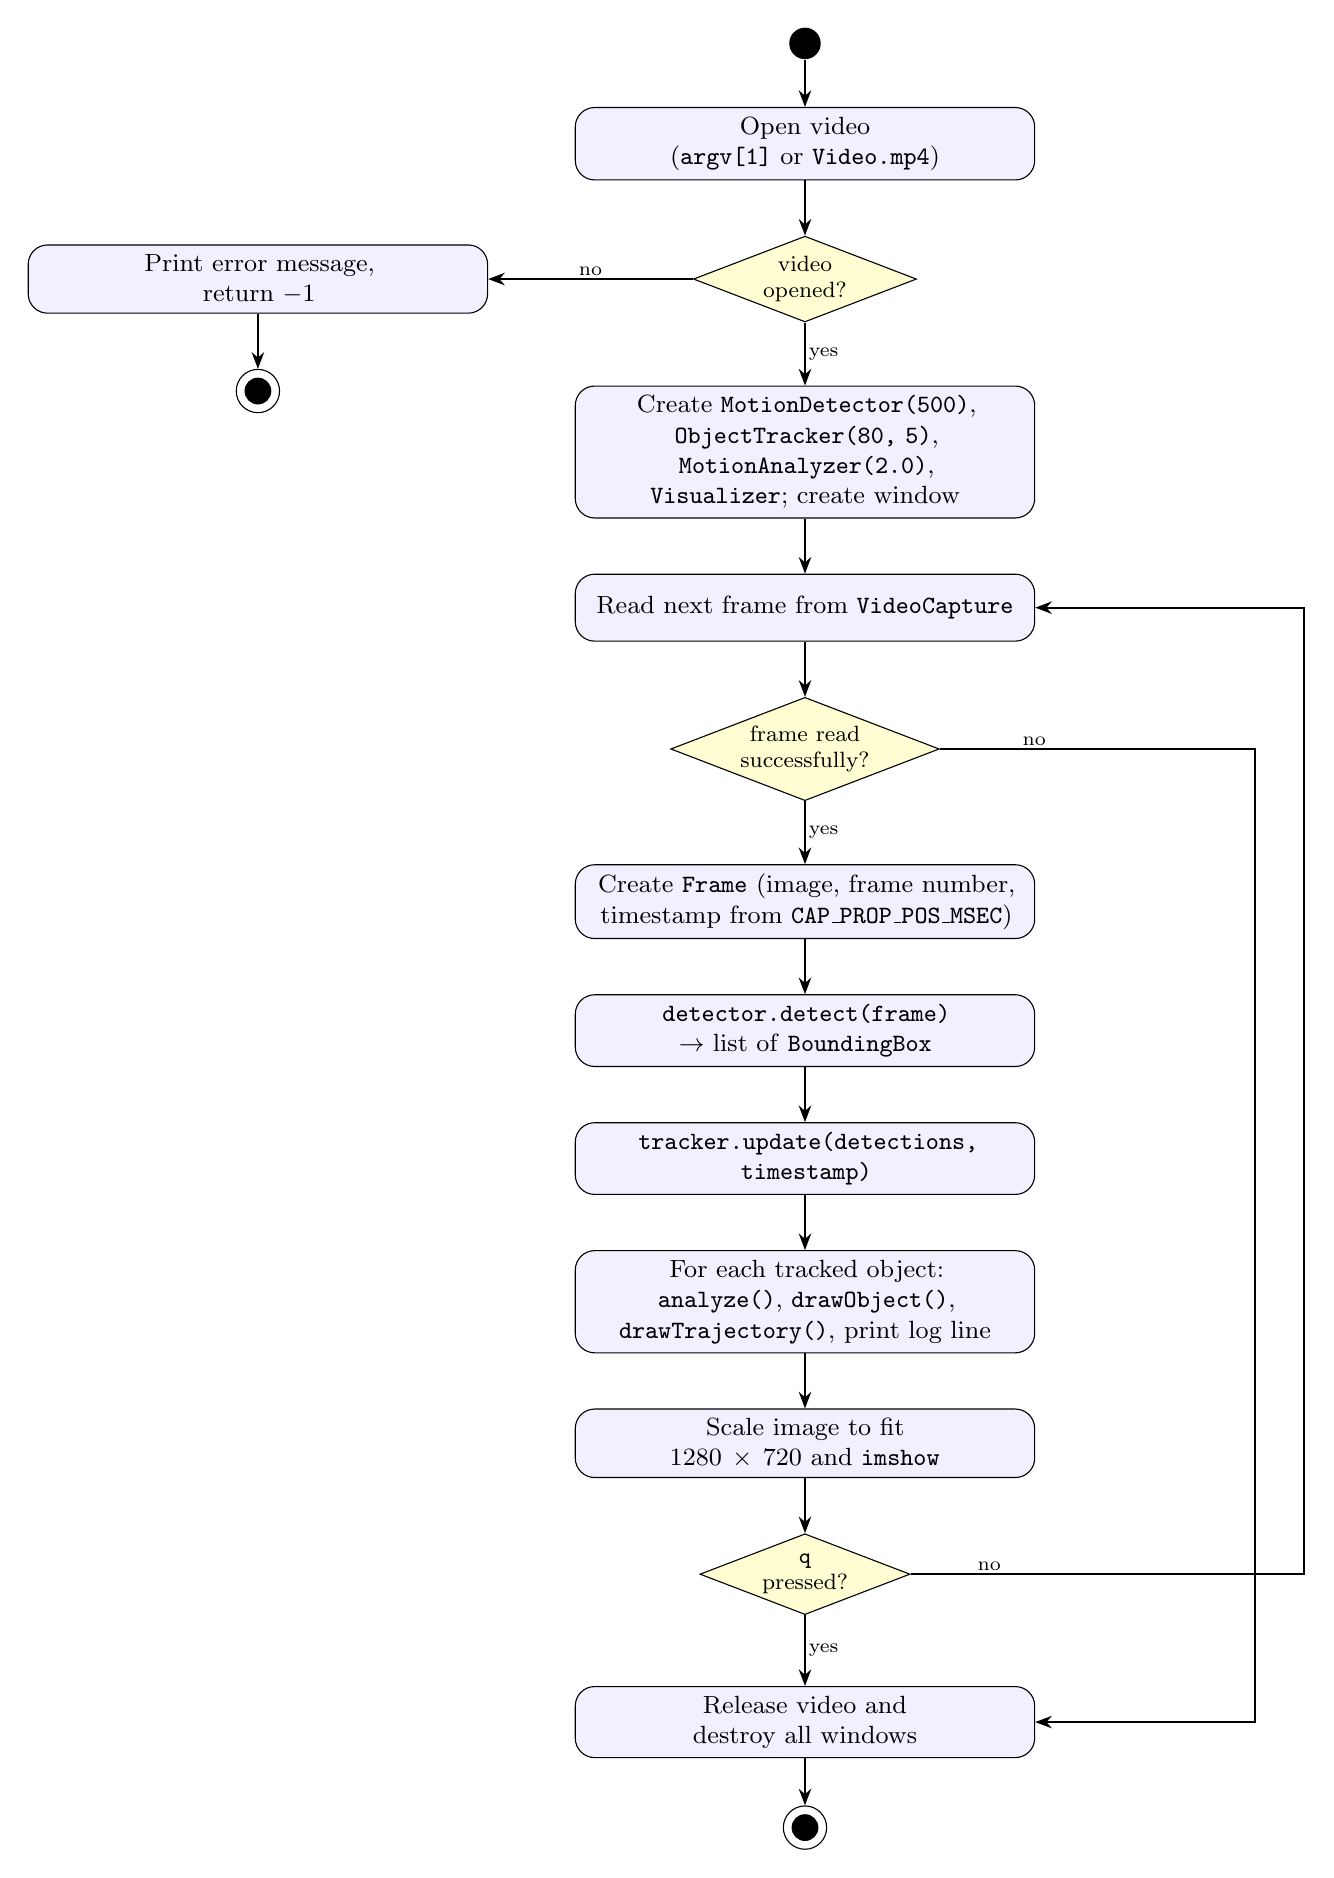
\begin{tikzpicture}[node distance=0.8cm]
\hyphenpenalty=10000 \exhyphenpenalty=10000
\node[startn] (s) {};
\node[act, below=0.6cm of s] (open) {Open video\\(\texttt{argv[1]} or \texttt{Video.mp4})};
\node[dec, below=0.7cm of open] (d1) {video\\opened?};
\node[act, left=2.6cm of d1] (err) {Print error message,\\return $-1$};
\node[endn, below=0.7cm of err] (e1) {};
\node[act, below=0.8cm of d1] (init) {Create \texttt{MotionDetector(500)}, \texttt{ObjectTracker(80, 5)}, \texttt{MotionAnalyzer(2.0)}, \texttt{Visualizer}; create window};
\node[act, below=0.7cm of init] (read) {Read next frame from \texttt{VideoCapture}};
\node[dec, below=0.7cm of read] (d2) {frame read\\successfully?};
\node[act, below=0.8cm of d2] (mk) {Create \texttt{Frame} (image, frame number, timestamp from \texttt{CAP\_PROP\_POS\_MSEC})};
\node[act, below=0.7cm of mk] (det) {\texttt{detector.detect(frame)} $\rightarrow$ list of \texttt{BoundingBox}};
\node[act, below=0.7cm of det] (trk) {\texttt{tracker.update(detections, timestamp)}};
\node[act, below=0.7cm of trk] (obj) {For each tracked object: \texttt{analyze()}, \texttt{drawObject()}, \texttt{drawTrajectory()}, print log line};
\node[act, below=0.7cm of obj] (disp) {Scale image to fit $1280\times720$ and \texttt{imshow}};
\node[dec, below=0.7cm of disp] (d3) {\texttt{q}\\pressed?};
\node[act, below=0.9cm of d3] (rel) {Release video and\\destroy all windows};
\node[endn, below=0.6cm of rel] (e2) {};
% flows
\draw[aflow] (s) -- (open);
\draw[aflow] (open) -- (d1);
\draw[aflow] (d1) -- node[gl, above] {no} (err);
\draw[aflow] (err) -- (e1);
\draw[aflow] (d1) -- node[gl, right] {yes} (init);
\draw[aflow] (init) -- (read);
\draw[aflow] (read) -- (d2);
\draw[aflow] (d2) -- node[gl, right] {yes} (mk);
\draw[aflow] (mk) -- (det);
\draw[aflow] (det) -- (trk);
\draw[aflow] (trk) -- (obj);
\draw[aflow] (obj) -- (disp);
\draw[aflow] (disp) -- (d3);
\draw[aflow] (d3) -- node[gl, right] {yes} (rel);
\draw[aflow] (rel) -- (e2);
% frame not read -> release
\draw[aflow] (d2.east) -- node[gl, above, pos=0.3] {no} ++(4.0,0) |- (rel.east);
% q not pressed -> loop back
\draw[aflow] (d3.east) -- node[gl, above, pos=0.2] {no} ++(5.0,0) |- (read.east);
\end{tikzpicture}}
\caption{Activity diagram of the main processing loop.}
\label{fig:activity-main}
\end{figure}

\begin{figure}[H]
\centering
\adjustbox{max width=\textwidth}{%
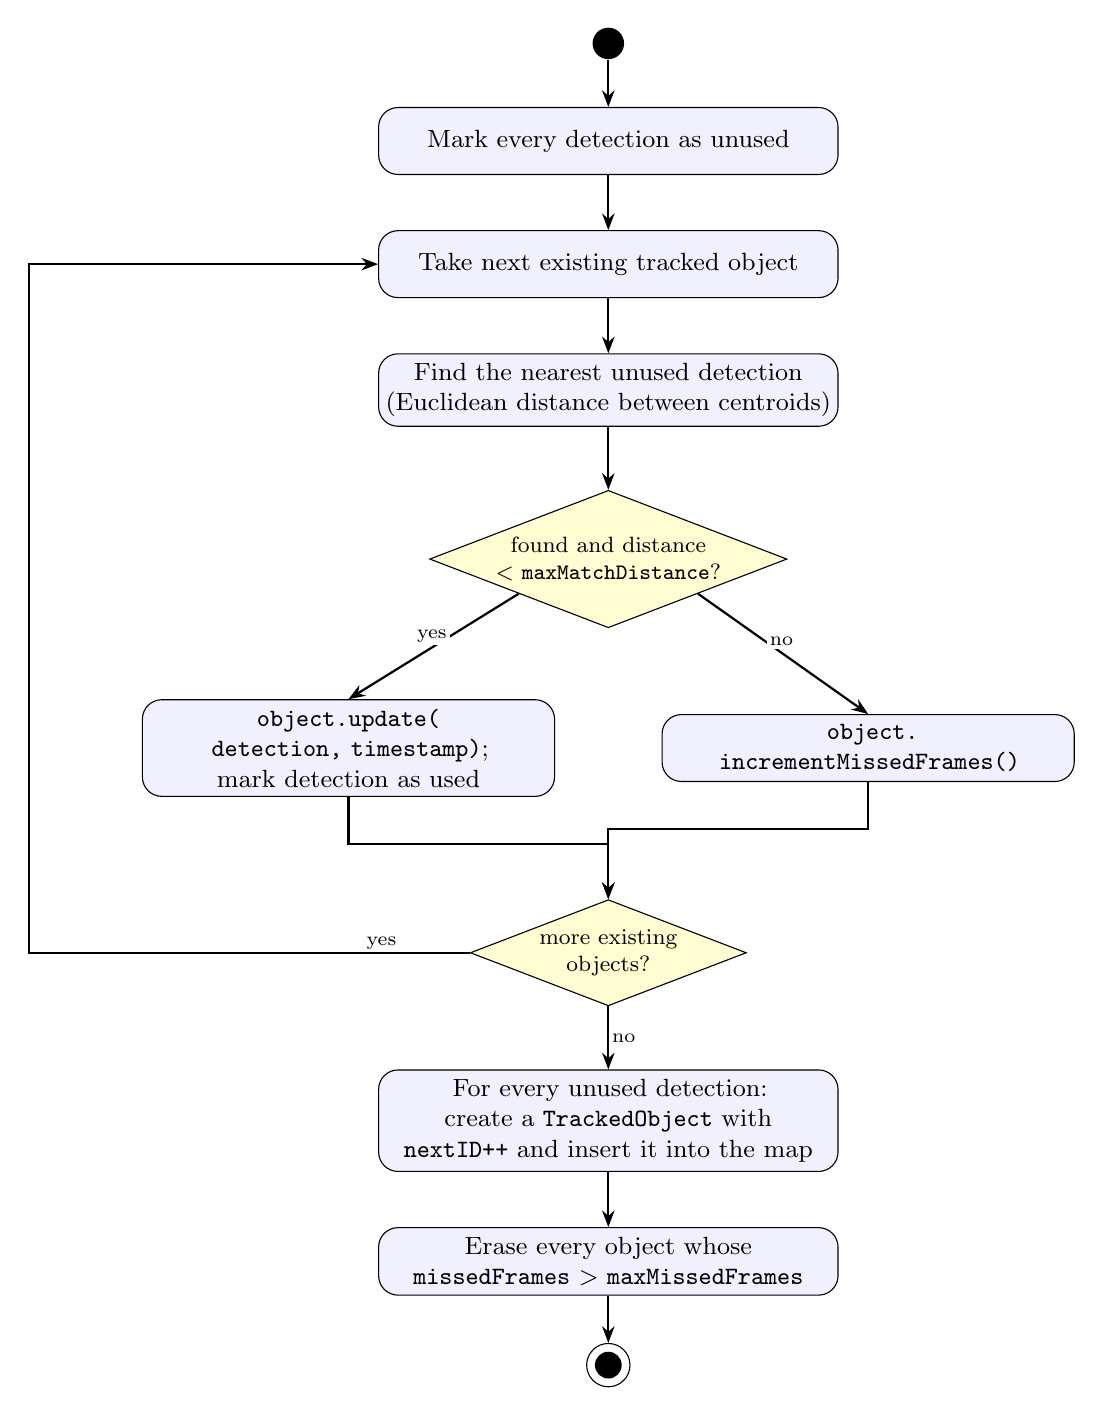
\begin{tikzpicture}[node distance=0.8cm]
\hyphenpenalty=10000 \exhyphenpenalty=10000
\node[startn] (s) {};
\node[act, below=0.6cm of s] (init) {Mark every detection as unused};
\node[act, below=0.7cm of init] (next) {Take next existing tracked object};
\node[act, below=0.7cm of next] (near) {Find the nearest unused detection (Euclidean distance between centroids)};
\node[dec, below=0.8cm of near] (d1) {found and distance\\$<$ \texttt{maxMatchDistance}?};
\node[act, text width=5.0cm] (yes) at ($(d1)+(-3.3,-2.4)$) {\texttt{object.update(}\\\texttt{detection, timestamp)};\\mark detection as used};
\node[act, text width=5.0cm] (no) at ($(d1)+(3.3,-2.4)$) {\texttt{object.}\\\texttt{incrementMissedFrames()}};
\node[dec] (d2) at ($(d1)+(0,-5.0)$) {more existing\\objects?};
\node[act, below=0.8cm of d2] (new) {For every unused detection: create a \texttt{TrackedObject} with \texttt{nextID++} and insert it into the map};
\node[act, below=0.7cm of new] (del) {Erase every object whose \texttt{missedFrames} $>$ \texttt{maxMissedFrames}};
\node[endn, below=0.6cm of del] (e) {};
% flows
\draw[aflow] (s) -- (init);
\draw[aflow] (init) -- (next);
\draw[aflow] (next) -- (near);
\draw[aflow] (near) -- (d1);
\draw[aflow] (d1.south west) -- node[gl, left, pos=0.4] {yes} (yes.north);
\draw[aflow] (d1.south east) -- node[gl, right, pos=0.4] {no} (no.north);
\draw[aflow] (yes.south) -- ++(0,-0.6) -| (d2.north);
\draw[aflow] (no.south) -- ++(0,-0.6) -| (d2.north);
\draw[aflow] (d2) -- node[gl, right] {no} (new);
\draw[aflow] (new) -- (del);
\draw[aflow] (del) -- (e);
\draw[aflow] (d2.west) -- node[gl, above, pos=0.2] {yes} ++(-5.6,0) |- (next.west);
\end{tikzpicture}}
\caption{Activity diagram of \texttt{ObjectTracker::update()}.}
\label{fig:activity-tracker}
\end{figure}

% =====================================================================
\section{Implementation Details}
% =====================================================================

\subsection{Motion Detection}
\texttt{MotionDetector::detect()} turns a \texttt{Frame} into a list of bounding boxes in five steps.
\begin{enumerate}
    \item \textbf{Background subtraction.} A MOG2 model (\texttt{cv::\allowbreak createBackground\allowbreak SubtractorMOG2()}, default parameters) is updated with the frame. MOG2 models each pixel as a mixture of Gaussians and marks it as background (0), shadow (127) or foreground (255).
    \item \textbf{Thresholding.} \texttt{cv::threshold(mask, mask, 200, 255, THRESH\_BINARY)} keeps only pixels that are clearly foreground. Because shadow pixels carry the value 127, they are discarded here.
    \item \textbf{Morphology.} Opening and then closing with a $5\times5$ rectangular kernel removes isolated specks and fills small holes inside objects.
    \item \textbf{Contours.} \texttt{cv::findContours} with \texttt{RETR\_EXTERNAL} extracts the outer contour of each connected region.
    \item \textbf{Area filter.} Contours with \texttt{contourArea} below \texttt{minimumArea} are ignored; for the rest, \texttt{cv::boundingRect} gives the \texttt{BoundingBox}.
\end{enumerate}

\begin{lstlisting}[caption={\texttt{MotionDetector::detect()} (core of the method).}, label={lst:detect}]
cv::Mat foregroundMask;
backgroundSubtractor->apply(image, foregroundMask);
// Remove noise
cv::threshold(foregroundMask, foregroundMask, 200, 255, cv::THRESH_BINARY);
cv::Mat kernel = cv::getStructuringElement(cv::MORPH_RECT, cv::Size(5, 5));
cv::morphologyEx(foregroundMask, foregroundMask, cv::MORPH_OPEN, kernel);
cv::morphologyEx(foregroundMask, foregroundMask, cv::MORPH_CLOSE, kernel);
std::vector<std::vector<cv::Point>> contours;
cv::findContours(foregroundMask, contours,
                 cv::RETR_EXTERNAL, cv::CHAIN_APPROX_SIMPLE);
for (const auto& contour : contours)
{
    double area = cv::contourArea(contour);
    if (area < minimumArea)
        continue;
    cv::Rect rect = cv::boundingRect(contour);
    BoundingBox box(rect.x, rect.y, rect.width, rect.height);
    detections.push_back(box);
}
\end{lstlisting}

\subsection{Object Tracking}
The tracker uses the centroid of each box, 
\begin{equation}
\mathbf{c} = \left(x + \frac{w}{2},\; y + \frac{h}{2}\right),
\end{equation}
and the Euclidean distance between an object's last centroid $\mathbf{c}_o$ and a detection's centroid $\mathbf{c}_d$,
\begin{equation}
d(\mathbf{c}_o,\mathbf{c}_d) = \sqrt{(c_{o,x}-c_{d,x})^2 + (c_{o,y}-c_{d,y})^2}.
\end{equation}
In every frame, each existing object (taken in ascending ID order) selects the closest detection that has not been used yet. If $d < d_{\max}$ (80 pixels by default), the object is updated with that detection; otherwise its missed-frame counter is incremented. Detections left unmatched start new objects with the next free ID. Finally, objects whose counter exceeds the limit (5 frames by default) are erased from the map. This is a simple \emph{greedy nearest-neighbour} strategy.

\begin{lstlisting}[caption={Matching loop of \texttt{ObjectTracker::update()}.}, label={lst:match}]
for (auto& pair : objects)
{
    TrackedObject& object = pair.second;
    double closestDistance = std::numeric_limits<double>::max();
    int closestIndex = -1;
    for (int i = 0; i < detections.size(); i++) {
        if (detectionUsed[i])
            continue;
        cv::Point2f objectCenter = object.getCurrentCentroid();
        cv::Point2f detectionCenter = detections[i].getCentroid();
        double dx = objectCenter.x - detectionCenter.x;
        double dy = objectCenter.y - detectionCenter.y;
        double distance = std::sqrt(dx * dx + dy * dy);
        if (distance < closestDistance) {
            closestDistance = distance;
            closestIndex = i;
        }
    }
    if (closestIndex != -1 && closestDistance < maxMatchDistance) {
        object.update(detections[closestIndex], timestamp);
        detectionUsed[closestIndex] = true;
    }
    else {
        object.incrementMissedFrames();
    }
}
\end{lstlisting}

\subsection{Motion Analysis}
From the previous and current centroids, the analyser computes the displacement $(\Delta x, \Delta y)$, the distance moved $s=\sqrt{\Delta x^2+\Delta y^2}$ and the speed
\begin{equation}
v = \frac{s}{\Delta t}\quad[\text{pixels/second}],
\end{equation}
where $\Delta t$ is the difference between the two video timestamps stored in the object (\texttt{getDeltaTime()}). Using real timestamps, instead of assuming a fixed frame rate, keeps the speed meaningful if the frame rate changes. The direction is decided by the dominant axis of motion and a movement threshold $\theta$ (2 pixels by default). Image $y$-coordinates grow downwards, so a negative $\Delta y$ means \texttt{UP}. The status is \texttt{MOVING} when $s>\theta$ and $v>0$, and otherwise \texttt{STATIONARY}, in which case the direction is also reset to \texttt{STATIONARY}.

\begin{lstlisting}[caption={Direction and status logic of \texttt{MotionAnalyzer::analyze()}.}, label={lst:analyze}]
std::string direction = "STATIONARY";
if (std::abs(dx) > std::abs(dy)) {
    if (dx > movementThreshold)       direction = "RIGHT";
    else if (dx < -movementThreshold) direction = "LEFT";
}
else {
    if (dy > movementThreshold)       direction = "DOWN";
    else if (dy < -movementThreshold) direction = "UP";
}
const std::string status = distance > movementThreshold && speed > 0.0
    ? "MOVING" : "STATIONARY";
if (status == "STATIONARY")
    direction = "STATIONARY";
object.setMotion(speed, direction, status);
\end{lstlisting}

\subsection{Visualisation and Display}
\texttt{Visualizer::drawObject()} draws the green bounding box, the red centroid dot and a white label placed just above the box (clamped so it stays inside the image), and \texttt{drawTrajectory()} joins the stored centroids with blue line segments. Before display, \texttt{main()} computes a scale factor $\min\{1,\;1280/\text{width},\;720/\text{height}\}$ and shrinks large frames with \texttt{cv::INTER\_AREA}, so that high-resolution videos fit on screen. Each log line printed to the console has the format
\begin{center}
\small\texttt{frame=<n> id=<id> x=<x> y=<y> speed\_px\_s=<v> direction=<d> status=<s> missed=<m>}
\end{center}

\subsection{Configuration Parameters}
\begin{table}[H]
\centering
\caption{Tunable parameters and their default values}
\label{tab:params}
\small
\begin{tabular}{@{}p{4.1cm}p{2.4cm}p{8.5cm}@{}}
\toprule
\textbf{Parameter} & \textbf{Value} & \textbf{Meaning}\\
\midrule
\texttt{minArea} (\texttt{MotionDetector}) & 500 px$^2$ & Smallest contour area accepted as an object\\
Foreground threshold & 200 & Removes shadow (127) and weak foreground pixels\\
Morphology kernel & $5\times5$ & Rectangular kernel for opening and closing\\
\texttt{maxDistance} (\texttt{ObjectTracker}) & 80 px & Largest centroid distance for a match\\
\texttt{maxMissed} (\texttt{ObjectTracker}) & 5 frames & Frames an unmatched object survives\\
\texttt{threshold} (\texttt{MotionAnalyzer}) & 2.0 px & Movement needed per frame to count as moving\\
Display limit & $1280\times720$ & Maximum size of the displayed window\\
\bottomrule
\end{tabular}
\end{table}

% =====================================================================
\section{Build and Execution}
% =====================================================================
The project is configured with CMake. \texttt{CMakeLists.txt} sets C++17, requires MSVC, locates OpenCV 5 through \texttt{OpenCV\_DIR} (default \texttt{C:/opencv/build}) and links the eight source files into one executable. For Visual Studio debugging it also adds the OpenCV \texttt{bin} directory to the \texttt{PATH} and sets the working directory to the source folder, so that the default \texttt{Video.mp4} is found.

\begin{lstlisting}[language={}, caption={Building and running the project (Developer PowerShell).}, label={lst:build}]
cmake --preset msvc-x64
cmake --build --preset msvc-debug

ObjectTrackingEngine.exe                 (plays Video.mp4)
ObjectTrackingEngine.exe path\to\clip.mp4
\end{lstlisting}

If the video cannot be opened, the program prints an error message and exits with code $-1$. While running, pressing \texttt{q} in the video window ends the program.

% =====================================================================
\section{Results and Screenshots}
% =====================================================================
The program was tested on a traffic-camera clip showing a multi-lane road with a bus stop. Figures~\ref{fig:res-single}--\ref{fig:res-crowded} show frames from the live window. The on-screen clock in the video (bottom right) gives the position in the clip.

\begin{figure}[H]
\centering
\includegraphics[width=0.92\textwidth]{images/ots_single_vehicle.jpg}
\caption{A single vehicle (ID 17, clip time 12:21:37) with its bounding box, centroid, label and a long blue trajectory. It is reported as \texttt{MOVING UP} at 67~px/s.}
\label{fig:res-single}
\end{figure}

\begin{figure}[H]
\centering
\includegraphics[width=0.92\textwidth]{images/ots_two_vehicles.jpg}
\caption{Two simultaneous objects (IDs 11 and 12, clip time 12:21:31) with independent IDs, labels and trajectories, both \texttt{MOVING UP}. The nearer car (ID 12) shows a larger pixel speed (152~px/s) than the farther one (ID 11, 145~px/s).}
\label{fig:res-two}
\end{figure}

\begin{figure}[H]
\centering
\includegraphics[width=0.92\textwidth]{images/ots_four_vehicles.jpg}
\caption{Four vehicles tracked at once (IDs 39, 40, 43 and 45, clip time 12:21:46). Vehicle 43, a taxi moving towards the right-hand lane, is labelled \texttt{MOVING RIGHT} at 135~px/s, while the others are \texttt{MOVING UP}.}
\label{fig:res-four}
\end{figure}

\begin{figure}[H]
\centering
\includegraphics[width=0.92\textwidth]{images/ots_crowded_scene.jpg}
\caption{A busier frame (clip time 12:22:01). The bus at the stop (ID 69) is labelled \texttt{STATIONARY}; other vehicles and a pedestrian at the right edge are tracked at the same time. Two overlapping boxes on the white car (IDs 77 and 80) show a case where one vehicle was detected as two regions.}
\label{fig:res-crowded}
\end{figure}

\subsection{Observations}
\begin{itemize}
    \item \textbf{Correct identities over time.} In the less crowded frames each vehicle keeps one ID and its trajectory follows the road lane, with a smooth path from the bottom of the image (nearer the camera) upwards.
    \item \textbf{Direction and status.} Most vehicles are labelled \texttt{MOVING UP}, matching the traffic direction, while the lane-changing taxi in Figure~\ref{fig:res-four} is reported as \texttt{MOVING RIGHT}, and the bus halted at the stop is reported as \texttt{STATIONARY}.
    \item \textbf{Perspective effect.} Speeds are measured in image pixels. Because the camera looks down the road, objects near the bottom of the image cover more pixels per second than distant ones moving equally fast, so values are comparable only for the same image region.
    \item \textbf{Challenging cases.} In Figure~\ref{fig:res-crowded}, a single car is covered by two boxes (IDs 77 and 80) and the label of ID~79 reads \texttt{MOVING STATIONARY}. The latter happens when the distance moved slightly exceeds the 2-pixel threshold while the dominant axis shows less than 2~pixels of motion, so the status becomes \texttt{MOVING} but no direction is assigned.
\end{itemize}

% =====================================================================
\section{Limitations and Future Work}
% =====================================================================
\subsection{Limitations}
\begin{itemize}
    \item \textbf{Greedy matching.} Objects choose detections one by one in ID order, without a global optimum. Two close objects, or an occlusion, can cause an ID switch.
    \item \textbf{No motion prediction.} The tracker compares a detection with an object's \emph{last} position; it does not predict where the object should be, so fast objects need a large matching radius.
    \item \textbf{Fragmented detections.} One large or partly occluded object can split into several contours, producing duplicate IDs (Figure~\ref{fig:res-crowded}).
    \item \textbf{Background absorption.} MOG2 slowly learns stationary objects into the background, so a vehicle that stops for a long time may eventually stop being detected.
    \item \textbf{Pixel units.} Speed is reported in pixels per second without perspective correction or calibration.
    \item \textbf{Direction labelling.} The rule uses only the dominant axis and a threshold, which can yield the combination \texttt{MOVING} / \texttt{STATIONARY} for very small motions.
    \item \textbf{Unbounded trajectories.} Each object stores its entire path; this is acceptable for short clips but grows for very long-lived objects.
\end{itemize}

\subsection{Future Work}
\begin{itemize}
    \item Replace greedy matching with the \textbf{Hungarian algorithm} for optimal assignment of detections to objects.
    \item Add a \textbf{Kalman filter} per object to predict its next position, smooth the trajectory and bridge short occlusions (as in SORT-style trackers).
    \item Introduce an abstract \texttt{Detector} base class with MOG2 and deep-learning (for example YOLO) implementations, which would also bring genuine inheritance and polymorphism into the project's own class hierarchy.
    \item Merge overlapping boxes and limit the stored trajectory length.
    \item Calibrate the camera (homography) to report speed in kilometres per hour, add object classification and per-lane counting, and save the annotated video to disk.
\end{itemize}

% =====================================================================
\section{Conclusion}
% =====================================================================
The Object Tracking Engine demonstrates how a non-trivial computer-vision pipeline can be organised into small, cohesive C++ classes. Detection, tracking, analysis and visualisation are separated behind simple interfaces; state is encapsulated; ownership is expressed through composition and standard containers; and the code uses constructors with default arguments, operator overloading, const-correctness and an abstract OpenCV interface. The results on real traffic footage show stable IDs, plausible trajectories and sensible direction and status labels, and the identified limitations point to clear next steps.

\section*{References}
\begin{enumerate}
    \item OpenCV documentation, \emph{Background Subtraction} and \emph{Structural Analysis and Shape Descriptors}. \url{https://docs.opencv.org/}
    \item Z.\ Zivkovic, ``Improved adaptive Gaussian mixture model for background subtraction,'' \emph{Proc.\ ICPR}, 2004.
    \item Z.\ Zivkovic and F.\ van der Heijden, ``Efficient adaptive density estimation per image pixel for the task of background subtraction,'' \emph{Pattern Recognition Letters}, 27(7), 2006.
    \item H.\ W.\ Kuhn, ``The Hungarian method for the assignment problem,'' \emph{Naval Research Logistics Quarterly}, 2(1--2), 1955.
    \item R.\ E.\ Kalman, ``A new approach to linear filtering and prediction problems,'' \emph{Journal of Basic Engineering}, 82(1), 1960.
    \item A.\ Bewley et al., ``Simple online and realtime tracking,'' \emph{Proc.\ IEEE ICIP}, 2016.
    \item B.\ Stroustrup, \emph{The C++ Programming Language}, 4th ed., Addison-Wesley, 2013.
\end{enumerate}

\end{document}
